% Options for packages loaded elsewhere
\PassOptionsToPackage{unicode}{hyperref}
\PassOptionsToPackage{hyphens}{url}
\PassOptionsToPackage{dvipsnames,svgnames,x11names}{xcolor}
%
\documentclass[
  letterpaper,
  DIV=11,
  numbers=noendperiod,
  oneside]{scrartcl}

\usepackage{amsmath,amssymb}
\usepackage{iftex}
\ifPDFTeX
  \usepackage[T1]{fontenc}
  \usepackage[utf8]{inputenc}
  \usepackage{textcomp} % provide euro and other symbols
\else % if luatex or xetex
  \usepackage{unicode-math}
  \defaultfontfeatures{Scale=MatchLowercase}
  \defaultfontfeatures[\rmfamily]{Ligatures=TeX,Scale=1}
\fi
\usepackage{lmodern}
\ifPDFTeX\else  
    % xetex/luatex font selection
\fi
% Use upquote if available, for straight quotes in verbatim environments
\IfFileExists{upquote.sty}{\usepackage{upquote}}{}
\IfFileExists{microtype.sty}{% use microtype if available
  \usepackage[]{microtype}
  \UseMicrotypeSet[protrusion]{basicmath} % disable protrusion for tt fonts
}{}
\makeatletter
\@ifundefined{KOMAClassName}{% if non-KOMA class
  \IfFileExists{parskip.sty}{%
    \usepackage{parskip}
  }{% else
    \setlength{\parindent}{0pt}
    \setlength{\parskip}{6pt plus 2pt minus 1pt}}
}{% if KOMA class
  \KOMAoptions{parskip=half}}
\makeatother
\usepackage{xcolor}
\usepackage[left=1in,marginparwidth=2.0666666666667in,textwidth=4.1333333333333in,marginparsep=0.3in]{geometry}
\setlength{\emergencystretch}{3em} % prevent overfull lines
\setcounter{secnumdepth}{-\maxdimen} % remove section numbering
% Make \paragraph and \subparagraph free-standing
\makeatletter
\ifx\paragraph\undefined\else
  \let\oldparagraph\paragraph
  \renewcommand{\paragraph}{
    \@ifstar
      \xxxParagraphStar
      \xxxParagraphNoStar
  }
  \newcommand{\xxxParagraphStar}[1]{\oldparagraph*{#1}\mbox{}}
  \newcommand{\xxxParagraphNoStar}[1]{\oldparagraph{#1}\mbox{}}
\fi
\ifx\subparagraph\undefined\else
  \let\oldsubparagraph\subparagraph
  \renewcommand{\subparagraph}{
    \@ifstar
      \xxxSubParagraphStar
      \xxxSubParagraphNoStar
  }
  \newcommand{\xxxSubParagraphStar}[1]{\oldsubparagraph*{#1}\mbox{}}
  \newcommand{\xxxSubParagraphNoStar}[1]{\oldsubparagraph{#1}\mbox{}}
\fi
\makeatother


\providecommand{\tightlist}{%
  \setlength{\itemsep}{0pt}\setlength{\parskip}{0pt}}\usepackage{longtable,booktabs,array}
\usepackage{calc} % for calculating minipage widths
% Correct order of tables after \paragraph or \subparagraph
\usepackage{etoolbox}
\makeatletter
\patchcmd\longtable{\par}{\if@noskipsec\mbox{}\fi\par}{}{}
\makeatother
% Allow footnotes in longtable head/foot
\IfFileExists{footnotehyper.sty}{\usepackage{footnotehyper}}{\usepackage{footnote}}
\makesavenoteenv{longtable}
\usepackage{graphicx}
\makeatletter
\def\maxwidth{\ifdim\Gin@nat@width>\linewidth\linewidth\else\Gin@nat@width\fi}
\def\maxheight{\ifdim\Gin@nat@height>\textheight\textheight\else\Gin@nat@height\fi}
\makeatother
% Scale images if necessary, so that they will not overflow the page
% margins by default, and it is still possible to overwrite the defaults
% using explicit options in \includegraphics[width, height, ...]{}
\setkeys{Gin}{width=\maxwidth,height=\maxheight,keepaspectratio}
% Set default figure placement to htbp
\makeatletter
\def\fps@figure{htbp}
\makeatother

% load packages
\usepackage{geometry}
\usepackage{xcolor}
\usepackage{eso-pic}
\usepackage{fancyhdr}
\usepackage{sectsty}
\usepackage{fontspec}
\usepackage{titlesec}

%% Set page size with a wider right margin
\geometry{a4paper, total={170mm,257mm}, left=20mm, top=20mm, bottom=20mm, right=50mm}

%% Let's define some colours
\definecolor{light}{HTML}{E6E6FA}
\definecolor{highlight}{HTML}{800080}
\definecolor{dark}{HTML}{330033}

%% Let's add the border on the right hand side 
\AddToShipoutPicture{% 
    \AtPageLowerLeft{% 
        \put(\LenToUnit{\dimexpr\paperwidth-3cm},0){% 
            \color{light}\rule{3cm}{\LenToUnit\paperheight}%
          }%
     }%
     % logo
    \AtPageLowerLeft{% start the bar at the bottom right of the page
        \put(\LenToUnit{\dimexpr\paperwidth-2.25cm},27.2cm){% move it to the top right
            \color{light}
\includegraphics[width=1.5cm]{_extensions/nrennie/PrettyPDF/logo.png}
          }%
     }%
}

%% Style the page number
\fancypagestyle{mystyle}{
  \fancyhf{}
  \renewcommand\headrulewidth{0pt}
  \fancyfoot[R]{\thepage}
  \fancyfootoffset{3.5cm}
}
\setlength{\footskip}{20pt}

%% style the chapter/section fonts
\chapterfont{\color{dark}\fontsize{20}{16.8}\selectfont}
\sectionfont{\color{dark}\fontsize{20}{16.8}\selectfont}
\subsectionfont{\color{dark}\fontsize{14}{16.8}\selectfont}
\titleformat{\subsection}
  {\sffamily\Large\bfseries}{\thesection}{1em}{}[{\titlerule[0.8pt]}]
  
% left align title
\makeatletter
\renewcommand{\maketitle}{\bgroup\setlength{\parindent}{0pt}
\begin{flushleft}
  {\sffamily\huge\textbf{\MakeUppercase{\@title}}} \vspace{0.3cm} \newline
  {\Large {\@subtitle}} \newline
  \@author
\end{flushleft}\egroup
}
\makeatother

%% Use some custom fonts
\setsansfont{Ubuntu}[
    Path=_extensions/nrennie/PrettyPDF/Ubuntu/,
    Scale=0.9,
    Extension = .ttf,
    UprightFont=*-Regular,
    BoldFont=*-Bold,
    ItalicFont=*-Italic,
    ]

\setmainfont{Ubuntu}[
    Path=_extensions/nrennie/PrettyPDF/Ubuntu/,
    Scale=0.9,
    Extension = .ttf,
    UprightFont=*-Regular,
    BoldFont=*-Bold,
    ItalicFont=*-Italic,
    ]
\KOMAoption{captions}{tableheading}
\makeatletter
\@ifpackageloaded{caption}{}{\usepackage{caption}}
\AtBeginDocument{%
\ifdefined\contentsname
  \renewcommand*\contentsname{Table of contents}
\else
  \newcommand\contentsname{Table of contents}
\fi
\ifdefined\listfigurename
  \renewcommand*\listfigurename{List of Figures}
\else
  \newcommand\listfigurename{List of Figures}
\fi
\ifdefined\listtablename
  \renewcommand*\listtablename{List of Tables}
\else
  \newcommand\listtablename{List of Tables}
\fi
\ifdefined\figurename
  \renewcommand*\figurename{Figure}
\else
  \newcommand\figurename{Figure}
\fi
\ifdefined\tablename
  \renewcommand*\tablename{Table}
\else
  \newcommand\tablename{Table}
\fi
}
\@ifpackageloaded{float}{}{\usepackage{float}}
\floatstyle{ruled}
\@ifundefined{c@chapter}{\newfloat{codelisting}{h}{lop}}{\newfloat{codelisting}{h}{lop}[chapter]}
\floatname{codelisting}{Listing}
\newcommand*\listoflistings{\listof{codelisting}{List of Listings}}
\makeatother
\makeatletter
\makeatother
\makeatletter
\@ifpackageloaded{caption}{}{\usepackage{caption}}
\@ifpackageloaded{subcaption}{}{\usepackage{subcaption}}
\makeatother
\makeatletter
\@ifpackageloaded{tcolorbox}{}{\usepackage[skins,breakable]{tcolorbox}}
\makeatother
\makeatletter
\@ifundefined{shadecolor}{\definecolor{shadecolor}{rgb}{.97, .97, .97}}{}
\makeatother
\makeatletter
\@ifundefined{codebgcolor}{\definecolor{codebgcolor}{named}{light}}{}
\makeatother
\makeatletter
\ifdefined\Shaded\renewenvironment{Shaded}{\begin{tcolorbox}[breakable, frame hidden, enhanced, boxrule=0pt, colback={codebgcolor}, sharp corners]}{\end{tcolorbox}}\fi
\makeatother
\makeatletter
\@ifpackageloaded{sidenotes}{}{\usepackage{sidenotes}}
\@ifpackageloaded{marginnote}{}{\usepackage{marginnote}}
\makeatother

\ifLuaTeX
  \usepackage{selnolig}  % disable illegal ligatures
\fi
\usepackage{bookmark}

\IfFileExists{xurl.sty}{\usepackage{xurl}}{} % add URL line breaks if available
\urlstyle{same} % disable monospaced font for URLs
\hypersetup{
  colorlinks=true,
  linkcolor={highlight},
  filecolor={Maroon},
  citecolor={Blue},
  urlcolor={highlight},
  pdfcreator={LaTeX via pandoc}}


\author{}
\date{}

\begin{document}

\pagestyle{mystyle}


Kyle Chayka,
``\href{https://www.newyorker.com/culture/infinite-scroll/how-the-internet-turned-us-into-content-machines}{How
The Internet Turned Us Into Content Machines}'' (\emph{New Yorker}, 4
June 2022)

\subsection{W2: Algorithm}\label{w2-algorithm}

{\marginnote{\begin{footnotesize}\href{https://www.kylechayka.com/}{Kyle
Chayka}, \textbf{Filterworld: How Algorithms Flattened
Culture}``\href{pdf/filterworld-intro.pdf}{Introduction}''
``\href{pdf/filterworld-ch1.pdf}{The Rise of Algorithmic
Recommendations}'' (ch.~1) See also:
``\href{https://www.newyorker.com/culture/infinite-scroll/the-banality-of-online-recommendation-culture}{The
Banality of Online Recommendation Culture}'' (\emph{New Yorker}, 30
October 2024)\end{footnotesize}}}

It can be safely assumed that, for better or worse, in light of the
events of the past twenty-four hours the Algorithm is probably the last
thing one anyone's mind right now! Nevertheless, I'm going to black-box
the election and its aftermath here and stay focused on the topic at
hand: the opening two chapters of Kyle Chayka's recent book on
algorithmic culture, \emph{Filterworld}.

The chapters themselves are so packed with insights and references to
other research sources that I'm not going to add to them here; I'm more
interested in hearing your own collective response to them and
discussing it with you in the coming week. Instead, I'll limit myself
here to connecting you to some of the sources on which Chayka's own book
is based, which provide an ideal starting point for anyone interested in
exploring the subject for your research project later in the course.

As with Kate Eichhorn's book about content or any of the other texts
that we're going to be dipping into in upcoming weeks, you might also be
interested in continuing with the book and writing a review of it for
the Book Report assignment due at the end of Week 5.

The first chapter of \emph{Filterworld} is essentially the extended of
mix of several articles that Chayka published as articles on his
\href{https://kylechayka.substack.com/p/on-algorithmic-anxiety}{Substack
blog} and subsequently in
\href{https://www.newyorker.com/culture/infinite-scroll/the-age-of-algorithmic-anxiety}{\emph{The
New Yorker}} (subscription required) in 2022. The Substack article in
particular is worth taking a closer look at because it references a
survey that Chayka conducted about algorithmic recommendation systems
that received 125 responses. I thought it might be interesting to assign
our group to answer some of the questions asked in the survey as a
starting point for our discussion.

Here are the main five questions, after those requesting name and
contact information. Since chapter 1 of \emph{Filterworld} provides a
definition of the term \textbf{algorithm} itself, I've also skipped that
one here:

\begin{itemize}
\tightlist
\item
  Has ``the algorithm,'' or algorithmic feeds, taken up more of your
  online experience over the years? What has that change felt like?
\item
  Do the algorithms of different platforms / feeds feel very different?
  Like TikTok vs Instagram, FB vs Twitter, Netflix vs Spotify\ldots{}
\item
  Have you had any particularly odd run-ins with algorithms or automated
  recommendations? Maybe it's eerily accurate Instagram ads (or terrible
  ones), getting served the same content as a friend, missing a Netflix
  show, or someone surprising popping up in your feed\ldots{} Describe
  anything that comes to mind.
\item
  If you are a creator (artist, musician, writer, YouTuber, whatever),
  do you ever feel pressure to mold your work in a certain way to fit
  with an algorithmic feed / platform? What is that pressure like?
\item
  Do you have any hacks / theories as to what makes a piece of content
  succeed in an algorithmic feed? Any tricks that you use or have used
  when you just want something to get attention?
\end{itemize}

You don't have to answer all of these questions, but for your Review
response this week, feel free to select one or two of them if you'd like
to respond. If it brings anything to mind, the third question, about
random or odd recommendations, might be the most interesting one of the
set.

I'm guessing that the section of Chayka's first chapter (not the
Introduction, the second, longer chapter) that you found most
interesting is about the concept of \textbf{algorithmic anxiety}, a term
that as he explains was used by Kate Crawford in 2013, was developed in
\href{https://networkcultures.org/contesting-capture-technology/}{Patricia
De Vries's blog} (well worth checking out!) for the
\href{https://networkcultures.org/}{Institute of Network Cultures}
website, and was the subject a 2018 academic paper about
\href{https://shagunjhaver.com/research/articles/jhaver-2018-airbnb/jhaver-2018-airbnb.pdf}{AirBnB}.De
Vries herself subsequently explored the subject in her pathbreaking
study
\href{https://networkcultures.org/blog/publication/tod33-algorithmic-anxiety-in-contemporary-art-a-kierkegaardian-inquiry-into-the-imaginary-of-possibility/}{\emph{Algorithmic
Anxiety in Contemporary Art}} (University of Amsterdam, 2020), available
as an open-source publication from the Institute's website.

As Chayka explains, De Vries's book emerged from her research on
contemporary digital artists whose work focuses on surveillance and
resistance to this, notably
\href{https://www.jillmagid.com/projects}{Jill Magid} and
\href{https://paglen.studio/}{Trevor Paglen}. For a survey of
contemporary internet art that includes chaptes on both of these
artists, see Lauren Cornell and Ed Halter's anthology,
\href{https://mitpress.mit.edu/9780262029261/mass-effect/}{\emph{Mass
Effect: Art and the Internet in the Twenty-First Century}} (Cambridge
,MA: MIT Press, 2015).

\marginnote{\begin{footnotesize}

\href{https://mitpress.mit.edu/9780262029261/mass-effect/}{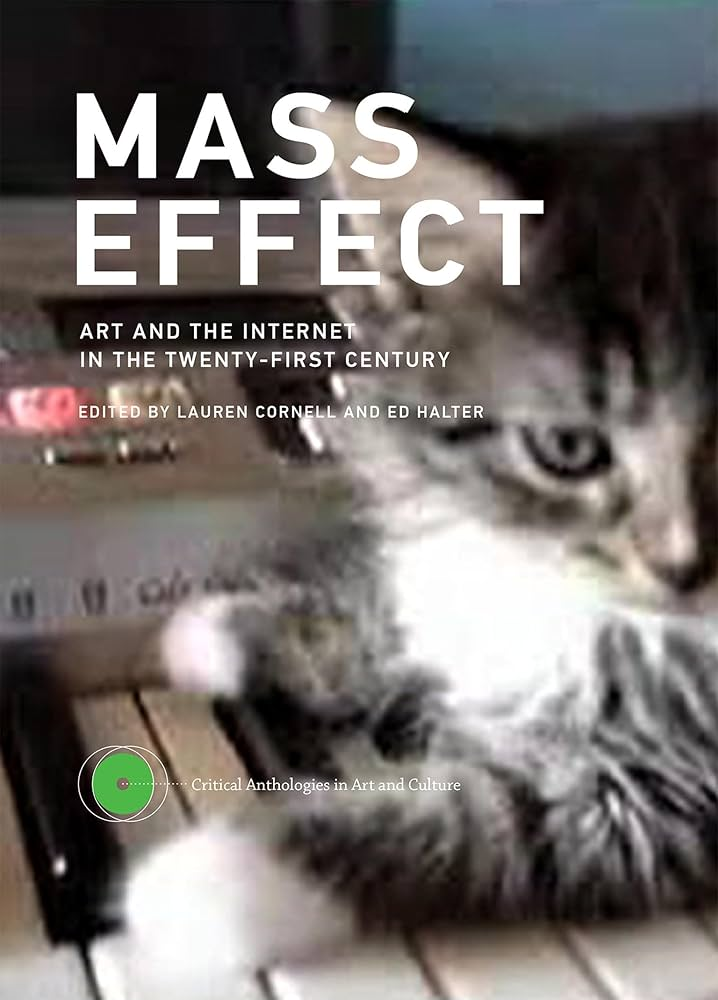
\includegraphics[width=2.08333in,height=\textheight]{img/mass-effect.jpg}}

\end{footnotesize}}

De Vries has a number of interesting presentations about internet art
and algorithmic culture on YouTube - I've created a
\href{https://www.youtube.com/playlist?list=PLx7AcHafElRiGpYPLRM29YzNMMEXyDqmh}{playlist}
for the course and have added them to it, and encourage you to take a
look. I'll be adding more YouTube sources to the playlist as the course
progresses, so add it to your bookmarks toolbar.

One other source mentioned in Chayka's chapter on algorithmic
recommendations is Taylor Lorenz's \emph{Washington Post} article about
the concept of \textbf{algospeak}, which I'm also linking to
here.{\marginnote{\begin{footnotesize}Taylor Lorenz,
``\href{https://www.washingtonpost.com/technology/2022/04/08/algospeak-tiktok-le-dollar-bean/}{Internet
`algospeak' is changing our language in real time, from `nip nops' to
`le dollar bean'}'' (\emph{Washington Post}, 8 April
2022).\end{footnotesize}}}

Taylor Lorenz is also the author of another interesting recent book
about contemporary internet culture.

\marginnote{\begin{footnotesize}

\href{https://www.simonandschuster.com/books/Extremely-Online/Taylor-Lorenz/9781982146863}{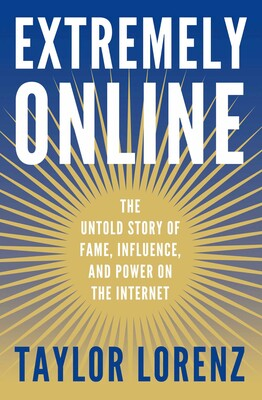
\includegraphics[width=2.08333in,height=\textheight]{img/extremely-online.jpg}}

\href{https://www.simonandschuster.com/books/Extremely-Online/Taylor-Lorenz/9781982146863}{\emph{Extremely
Online: The Untold Story of Fame, Influence, and Power on the Internet}}
(New York: Simon \& Schuster, 2023).

\end{footnotesize}}

Well that should keep you busy for a week or two! Look forward to
discussing the \emph{Filterworld} chapters and any other of the above
sources with you in the coming week!

\begin{center}\rule{0.5\linewidth}{0.5pt}\end{center}




\end{document}
